

\tikzset{every picture/.style={line width=0.75pt}} %set default line width to 0.75pt        
\begin{center}
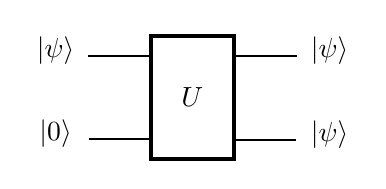
\begin{tikzpicture}[x=0.75pt,y=0.75pt,yscale=-1,xscale=1]
%uncomment if require: \path (0,300); %set diagram left start at 0, and has height of 300

%Shape: Rectangle [id:dp5049814893934905] 
\draw  [line width=1.5]  (220,120.5) -- (259.75,120.5) -- (259.75,179.5) -- (220,179.5) -- cycle ;
%Straight Lines [id:da7877497388492118] 
\draw    (189.75,130) -- (219.75,130) ;


%Straight Lines [id:da009334325250696995] 
\draw    (190.25,170) -- (220.25,170) ;


%Straight Lines [id:da9491833456963361] 
\draw    (260.25,130) -- (290.25,130) ;


%Straight Lines [id:da9179785583004338] 
\draw    (259.75,170.5) -- (289.75,170.5) ;



% Text Node
\draw (174,127.5) node   {$|\psi \rangle $};
% Text Node
\draw (174,167.5) node   {$|0\rangle $};
% Text Node
\draw (306,127.5) node   {$|\psi \rangle $};
% Text Node
\draw (306,168) node   {$|\psi \rangle $};
% Text Node
\draw (239.88,150) node   {$U$};


\end{tikzpicture}
\end{center}